\begin{pastexam}[label={px:nsysu-115-osds-02}]{中山資工所甲組 115 學年度 第 6 題}
（問答；10 分）

(10\%) Given the inorder traversal ABCDEFGHIJ and the postorder traversal ABDCGIHJFE of a binary
tree, determine the preorder traversal.
\end{pastexam}

\begin{pastsoln}
答案：前序是 \texttt{ECBADFJHGI}。

做法（資結書第~7.4~節）：後序的最後一個是根；在中序裡找到根，左邊是左子樹、右邊是右子樹；
後序裡左子樹的節點個數和中序一樣，照個數切開，兩邊遞迴。 每一步寫「中序｜後序 $\Rightarrow$ 根」：
\begin{enumerate}
\item ABCDEFGHIJ｜ABDCGIHJF\textbf{E} $\Rightarrow$ 根 E。 左子樹中序 ABCD（後序 ABDC），右子樹
中序 FGHIJ（後序 GIHJF）。
\item ABCD｜ABD\textbf{C} $\Rightarrow$ 根 C。 左子樹 AB（後序 AB），右子樹 D。
\item AB｜A\textbf{B} $\Rightarrow$ 根 B，A 在中序裡在 B 左邊，是 B 的左子節點。
\item FGHIJ｜GIHJ\textbf{F} $\Rightarrow$ 根 F。 F 在中序最前面，左子樹空，右子樹 GHIJ（後序 GIHJ）。
\item GHIJ｜GIH\textbf{J} $\Rightarrow$ 根 J。 J 在中序最後，右子樹空，左子樹 GHI（後序 GIH）。
\item GHI｜GI\textbf{H} $\Rightarrow$ 根 H，左子節點 G、右子節點 I。
\end{enumerate}
\begin{center}
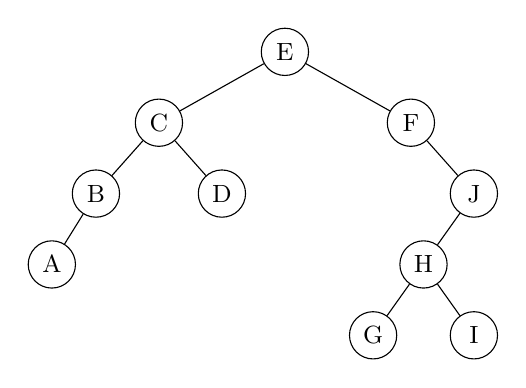
\begin{tikzpicture}[x=0.8cm,y=0.9cm,v/.style={circle,draw,minimum size=6mm,inner sep=0pt,font=\small}]
\node[v] (E) at (0,0) {E};
\node[v] (C) at (-2,-1) {C};
\node[v] (F) at (2,-1) {F};
\node[v] (B) at (-3,-2) {B};
\node[v] (D) at (-1,-2) {D};
\node[v] (J) at (3,-2) {J};
\node[v] (A) at (-3.7,-3) {A};
\node[v] (H) at (2.2,-3) {H};
\node[v] (G) at (1.4,-4) {G};
\node[v] (I) at (3,-4) {I};
\draw (E)--(C) (E)--(F) (C)--(B) (C)--(D) (B)--(A) (F)--(J) (J)--(H) (H)--(G) (H)--(I);
\end{tikzpicture}
\end{center}
檢查：這棵樹的中序（左、根、右）是 A B C D E F G H I J，後序（左、右、根）是
A B D C G I H J F E，都和題目相同。 中序和後序可以唯一決定一棵二元樹（節點互不相同時），所以
這就是那棵樹。 前序（根、左、右）：E，左子樹 C B A D，右子樹 F J H G I，合起來
\[
\mathtt{E\,C\,B\,A\,D\,F\,J\,H\,G\,I}.
\]
\end{pastsoln}
